\documentclass[11pt,UTF8]{ctexart}

\usepackage[margin=2cm,a4paper]{geometry}
%\usepackage[left=0.75in,top=0.6in,right=0.75in,bottom=1.0in,a4paper]{geometry}


\setmainfont{Caladea}
%% 也可以选用其它字库:
% \setCJKmainfont[%
%   ItalicFont=AR PL KaitiM GB,
%   BoldFont=Noto Sans CJK SC,
% ]{Noto Serif CJK SC}
% \setCJKsansfont{Noto Sans CJK SC}
% \renewcommand{\kaishu}{\CJKfontspec{AR PL KaitiM GB}}
\setCJKsansfont{Noto Sans CJK TC}

\usepackage{minted}
\usepackage[breaklinks]{hyperref}

% Picture
% 导言区的此三行无变化
\usepackage{graphicx}
\usepackage{float} 
\usepackage{subfigure}
% 以下是新增的自定义格式更改
\usepackage[]{caption2} %新增调用的宏包
\renewcommand{\figurename}{Fig.} %重定义编号前缀词
\renewcommand{\captionlabeldelim}{.~} %重定义分隔符
 %\roman 是罗马数字编号,\alph是默认的字母编号,\arabic是阿拉伯数字编号,可按需替换下一行的相应位置
\renewcommand{\thesubfigure}{(\roman{subfigure})}%此外,还可设置图编号显示格式,加括号或者不加括号
\makeatletter \renewcommand{\@thesubfigure}{\thesubfigure \space}%子图编号与名称的间隔设置
\renewcommand{\p@subfigure}{} \makeatother

% Math
\usepackage {mathtools}
\usepackage{amssymb}

% Code
\usepackage{listings}
\usepackage{xcolor}
\lstset{
    % backgroundcolor=\color{red!50!green!50!blue!50},
    % 程式碼塊背景色為淺灰色
    rulesepcolor= \color{gray}, % 程式碼塊邊框顏色
    breaklines=true,  % 程式碼過長則換行
    numbers=left, % 行號在左側顯示
    numberstyle= \small,% 行號字型
    % eywordstyle= \color{red,% 關鍵字顏色
    commentstyle=\color{gray}, % 註釋顏色
    frame=shadowbox % 用方框框住程式碼塊
    }

\usepackage{hyperref}

\title{计算机视觉作业}
\author{干皓丞,2101212850, 信息工程学院}

\begin{document}
\maketitle


\section{题目}

Pytorch 程式码如下
\\
	\begin{lstlisting}[language={python}]
import torch
torch.manual_seed(0)
x = torch.randn(10,4, requires_grad=True)
W = torch.randn(4,4, requires_grad=True)
y = torch.randn(10,4, requires_grad=True)
	\end{lstlisting}


目标函数 :

$$f={||\ max(\ XW,)\ -\ Y\ ||}_F^2$$

手推写出已下表达式,并用 Pytorch 进行实现。
$$ (1)\quad \frac{\partial f}{\partial W}  \quad (2)\quad \frac{\partial f}{\partial X} \quad (3)\quad \frac{\partial f}{\partial Y}$$

\section{数学式定义与程式码的数学意义说明}

(1) 斜变函数与单位阶跃函数

$$f={||\ max(\ XW,)\ -\ Y\ ||}_F^2$$

目标函数当中的 max(x,0) 表示的是单位斜变函数,也就是所谓的整流线性单位函式(Rectified Linear Unit, ReLU),该函数特性在小于时归零,大于零保持原值,但当进行微分时,会变成单位阶跃函数(Heaviside step function),函数小于零时为零,大于零时则为一,其两者数学图形如下(来源为 Wikipedia)。

\begin{figure}[H]
\centering  %图片全局居中
\subfigure[单位斜变函数]{
\label{Fig.sub.1}
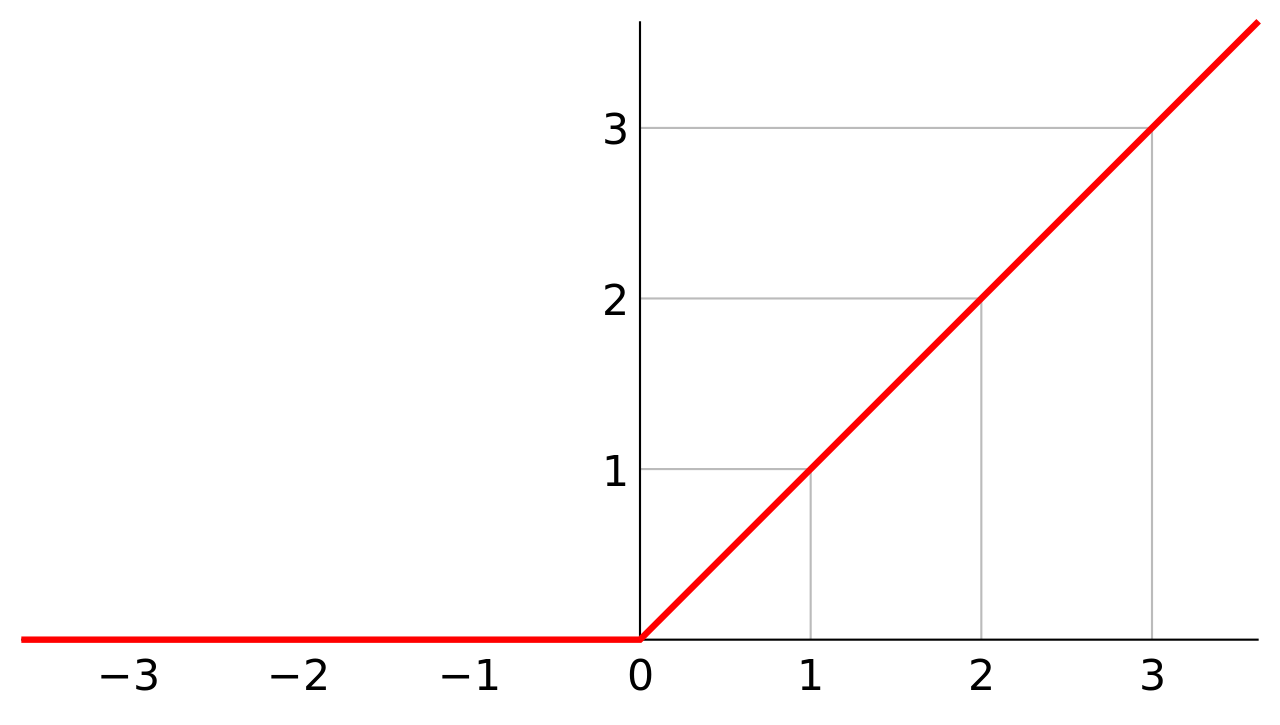
\includegraphics[width=0.45\textwidth]{r1.png}}
\subfigure[单位阶跃函数]{
\label{Fig.sub.2}
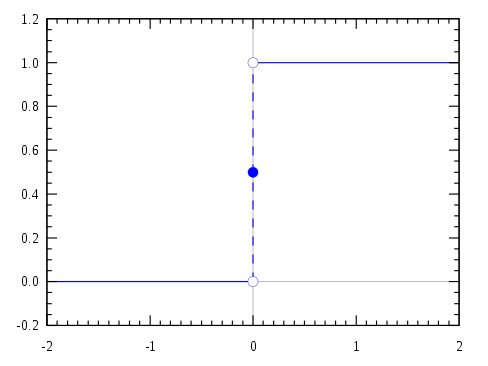
\includegraphics[width=0.45\textwidth]{r2.png}}
\caption{单位斜变函数与单位阶跃函数}
\label{Fig.main}
\end{figure}

而单位斜变函数在此表示为 $R\ (x)$ ,单位阶跃函数函数在此表示为 $H\ (x)$ ,
同时两者各自的函数范围与二者之间的微分关系如下 :

$$ R\ (x)=\left\{
\begin{aligned}
\quad x,\quad x\quad\geq\quad0 \\
\quad 0,\quad x\quad\textless\quad0 \\
\end{aligned}
\right.
\quad; \quad 
H\ (x)=\left\{
\begin{aligned}
\quad 0,\quad x\quad\textless\quad 0 \\
\quad 1,\quad x\quad\geq\quad 0 \\
\end{aligned}
\right.
\quad; \quad 
 R'\ (x)=  H\ (x),\quad if\quad x \neq 0
$$
\\
(2) 程式码中的数学意义
\\
	\begin{lstlisting}[language={python}]
import torch
torch.manual_seed(0)
x = torch.randn(10,4, requires_grad=True)
W = torch.randn(4,4, requires_grad=True)
y = torch.randn(10,4, requires_grad=True)
	\end{lstlisting}

程式码当中的 W 、x、y 在数学上分别代表了 W 、X、Y 三个矩阵,W 為 4 X 4 大小的矩陣,X 与 Y 矩阵皆为 10 X 4 大小的矩阵,而 Pytorch 则会随机产生矩阵中的值。

$$X\ =\ \left[\begin{matrix}x_{11}&\cdots&x_{14}\\\vdots&\ddots&\vdots\\x_{10\ 1}&\cdots&x_{10\ 4}\\\end{matrix}\right]\quad, \quad Y\ =\ \left[\begin{matrix}y_{11}&\cdots&y_{14}\\\vdots&\ddots&\vdots\\y_{10\ 1}&\cdots&y_{10\ 4}\\\end{matrix}\right]\quad, \quad W\ =\ \left[\begin{matrix}w_{11}&\cdots&w_{14}\\\vdots&\ddots&\vdots\\w_{41}&\cdots&w_{44}\\\end{matrix}\right]$$

\newpage

\section{数学推导证明}

$$f={||\ max(\ XW,)\ -\ Y\ ||}_F^2 \rightarrow f\ =tr({(max(XW,0)-\ Y)}^T.(max(XW,0)-\ Y))$$

%% \because  \therefore

$$\therefore\quad df\ =tr({-{dY}^T.(max(XW,0)-\ Y)-(max(XW,0)-\ Y)}^T.dY)$$

$$=tr({-2(max(XW,0)-\ Y)}^T.dY)$$

$$\therefore\quad \frac{df}{dY}\ =\ -2(max(XW,0)-\ Y)$$

$$\because\quad  f\ =tr({(XW\odot\varepsilon(XW)-\ Y)}^T.(XW\odot\varepsilon(XW)-\ Y))$$

其中 $\varepsilon$ 函数,在此也就表示上节所述的单位斜变函数与单位阶跃函数,$\varepsilon‘= 0$,而符号 $\odot$ 则表示逐元素对应相乘。

$$\therefore\quad df\ =tr({(XdW\odot\varepsilon(XW))}^T.(max(XW,0)-\ Y)+{(max(XW,\ 0)-Y)}^T.(XdW\odot\varepsilon(XW))$$

$$=tr({2(max(XW,\ 0)-Y)}^T.\varepsilon(XW)\odot XdW)$$

$$=tr({2((max(XW,\ 0)-Y)\odot\varepsilon(XW))}^T.XdW)$$

$$\therefore\quad \frac{df}{dW}\ =\ 2X^T((max(XW,0)-\ Y)\mathrm{\odot\varepsilon(XW)})$$

$$df\ =tr({((max(XW,\ 0)-Y)\odot\varepsilon(XW))}^T.dX.W)$$

$$=tr(2W{((max(XW,\ 0)-Y)\odot\varepsilon(XW))}^T.dX)$$

$$\therefore\quad \frac{df}{dX}\ =\ 2((max(XW,0)-\ Y)\mathrm{\odot\varepsilon(XW)}).W^T$$

\newpage

\section{Pytorch 程式码实现}

程式码可以在 GitHub 項目(kancheng/kan-cs-report-in-2021)找到,详见 math.ipynb 档案。


(1) Pytorch 实验资料

下列为 Pytorch 所产生矩阵实验资料。
\newline

	\begin{lstlisting}[language={python}]
import torch
torch.manual_seed(0)
x = torch.randn(10,4, requires_grad=True)
W = torch.randn(4,4, requires_grad=True)
y = torch.randn(10,4, requires_grad=True)
print(x)
print(y)
print(W)
	\end{lstlisting}
	
\begin{figure}[H]
\centering 
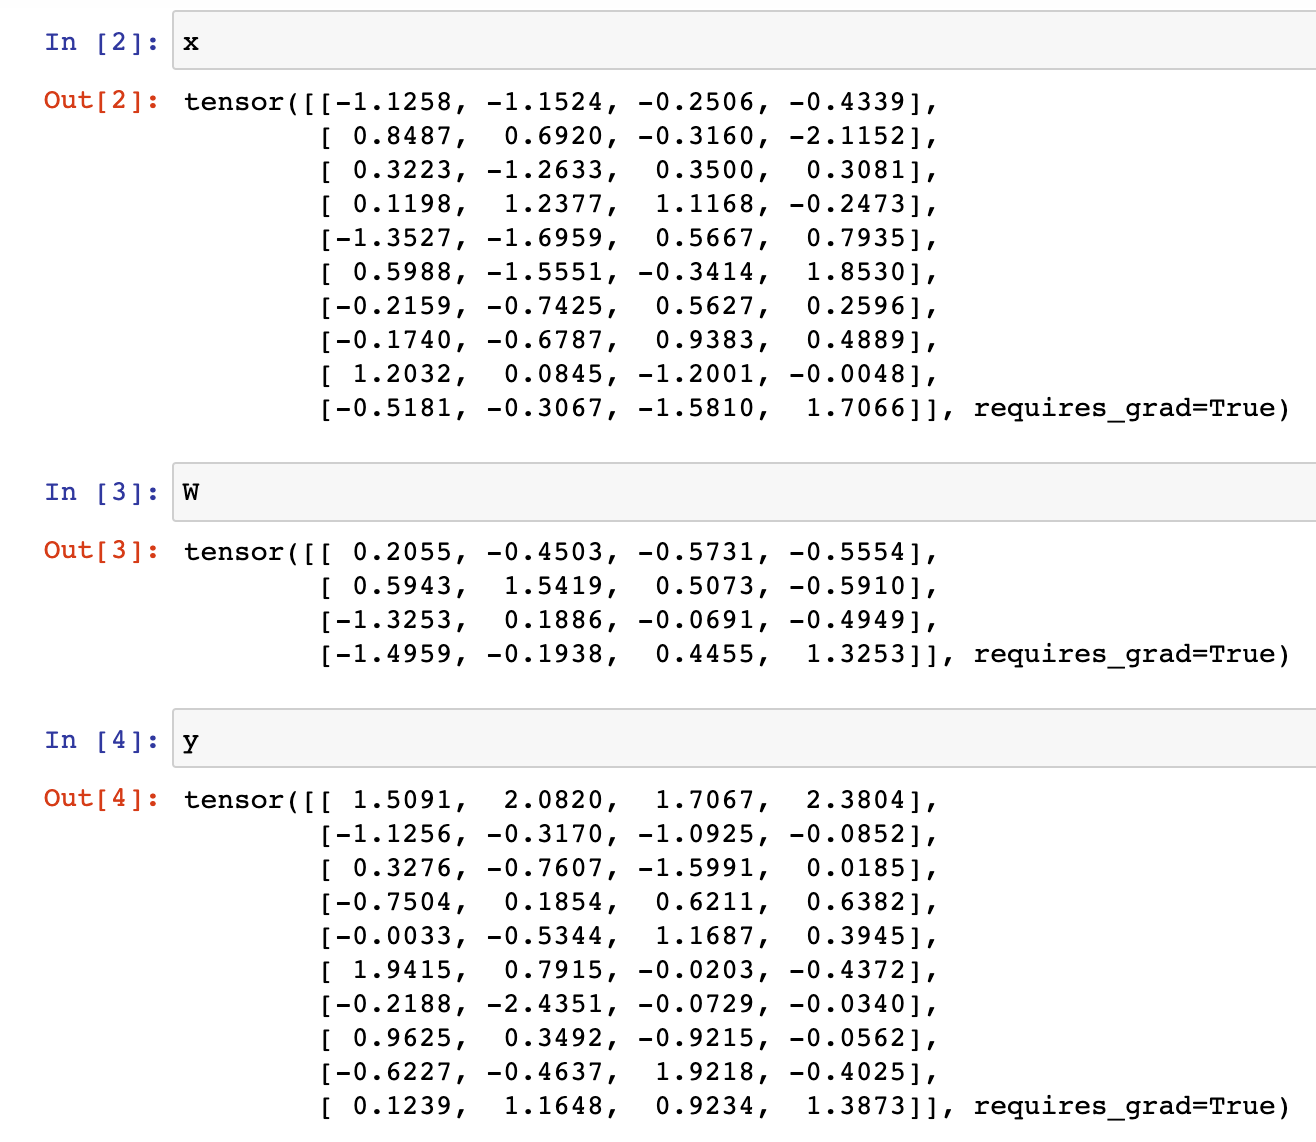
\includegraphics[width=0.7\textwidth]{c1.png} 
\caption{Pytorch 矩阵}
\label{Code.1}
\end{figure}

\newpage

(2) 直接微分求导
\newline

下列为 Pytorch 程式码,此程式码根据目标函数 $f = ||max(XW,0)-Y||^2_F $ 与相关数学式 $f = ||\hat{Y}-Y||^2_F $、$\hat{Y} = max(Z,0)$、 $Z = XW$ ,來进行微分求导。
\newline


	\begin{lstlisting}[language={python}]
# f = (torch.clamp(x.mm(W), 0) - y).pow(2).sum()
f1 = (torch.clamp(x.mm(W), 0) - y).pow(2).sum()
# torch.clamp 讓小於零的值,賦值為零。
print(f1)

# XW 矩陣乘法
z = x.mm(W)
print(z)
# 測試 torch 寫法
# test = torch.mm( x, W)
# print(test)

# ReLU
m = torch.nn.ReLU()
tm = m(z)
y_hat = tm
# 建立第二次式
f2 = (y_hat - y).pow(2).sum()

print(f2)

# W.grad.zero_()
print(W.grad)

# f.backward()
f2.backward()

print(W.grad)
print(y.grad)
print(x.grad)
	\end{lstlisting}
	
\newpage

下列为 Pytorch 程式码,根据目标函数所产生的微分求导结果。
\newline

\begin{figure}[H]
\centering 
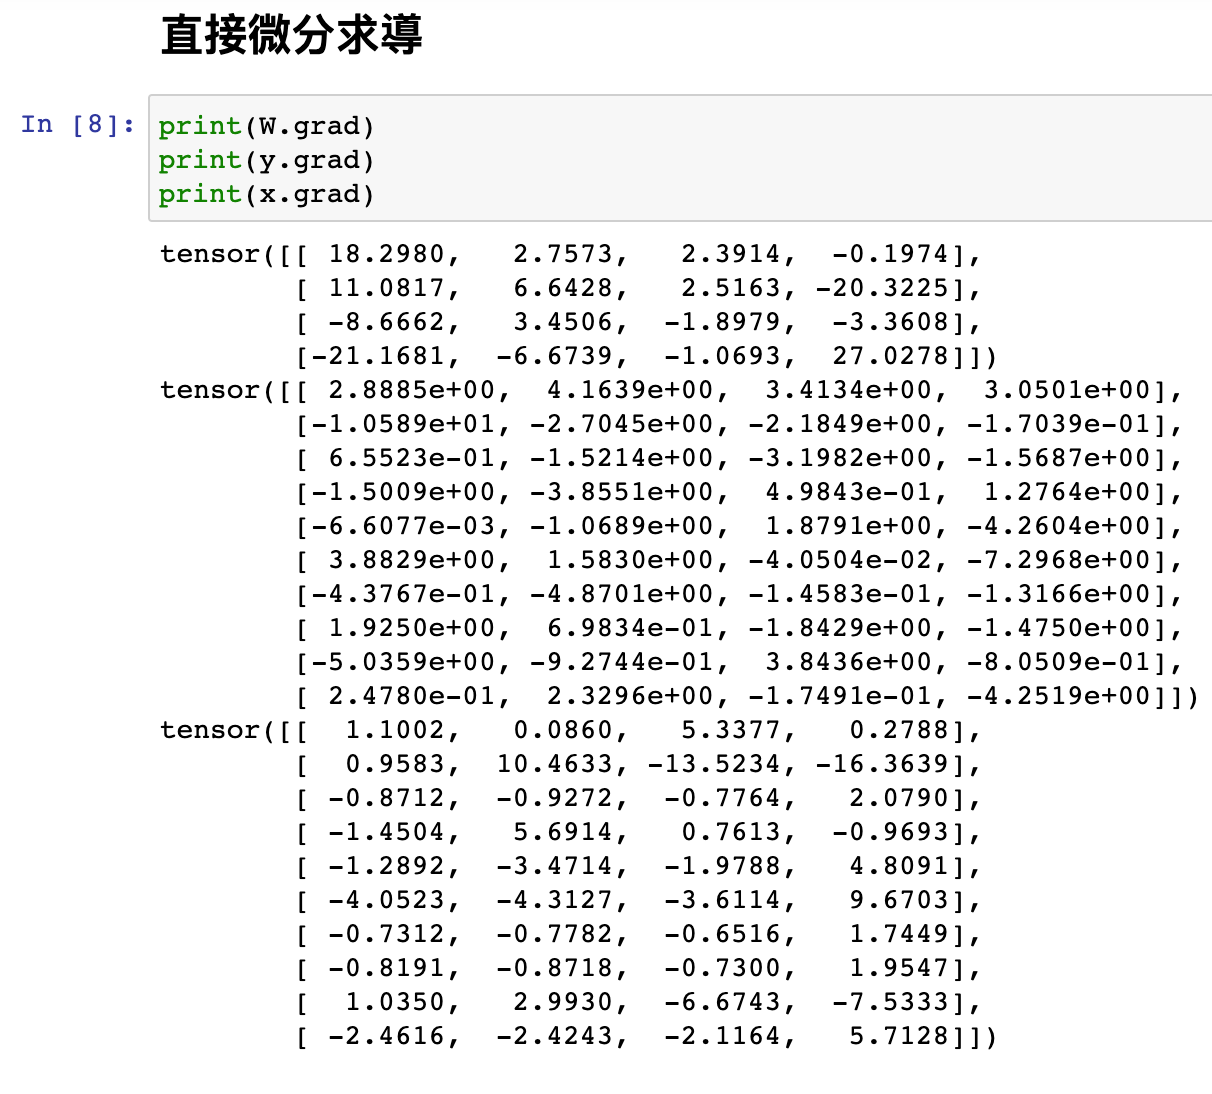
\includegraphics[width=0.7\textwidth]{c2.png} 
\caption{Pytorch 直接求导}
\label{Code.2}
\end{figure}

\newpage

(3) 公式推导求导
\newline

下列为 Pytorch 程式码,此程式码根据目标函数 $f = ||max(XW,0)-Y||^2_F $ 与相关数学式 $f = ||\hat{Y}-Y||^2_F $、$\hat{Y} = max(Z,0)$、 $Z = XW$ ,跟前章数学推导后的公式进行求导。

	\begin{lstlisting}[language={python}]
y_grad = -2*(y_hat-y)
print(y_grad)

v = abs(x.mm(W)* 0)
g = torch.heaviside(input =x.mm(W), values = v)
x_grad = 2*(torch.mul((y_hat-y),g)).mm(torch.t(W))
print(x_grad)

W_grad = 2*torch.t(x).mm(torch.mul((y_hat-y),g))
print(W_grad)

	\end{lstlisting}


\begin{figure}[H]
\centering 
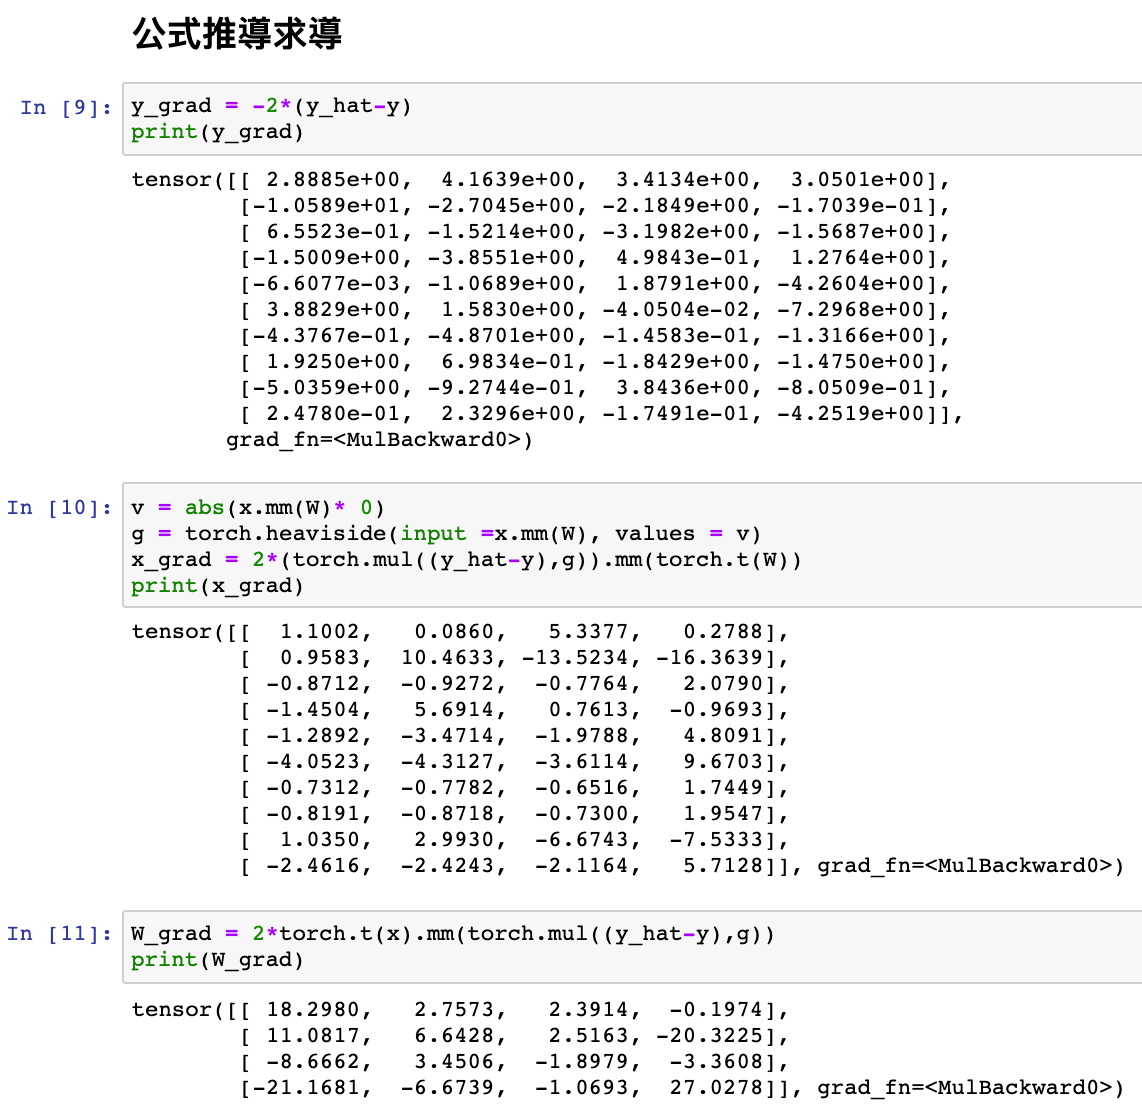
\includegraphics[width=0.7\textwidth]{c3.png} 
\caption{Pytorch 公式求导}
\label{Code.3}
\end{figure}

\clearpage

\end{document}